% Ready-to-paste reviewer-response draft for the revised distribution diagnostic.
\subsection*{A2. Train/test overlap for FT-600K}

\noindent\textbf{Reviewer comment.}
\begin{quote}
\itshape
``Rule out train/test overlap for FT-600K: report the minimum SOAP-distance (or RMSD) between each in-gap NEB image and its nearest fine-tuning frame, or re-run FT-600K with the NEB-adjacent trajectory segment excluded, and confirm the 0.16 eV result survives.''
\end{quote}

\noindent\textbf{Response.}

We agree that trajectory provenance and geometric proximity must be audited separately from pointwise RMSE. The FT-600K fine-tuning source consists of 600~K AIMD trajectories; NEB output, NEB optimization frames, and NEB-adjacent path segments were not part of the declared fine-tuning source. We therefore rebuilt the split at the source-trajectory level rather than by a frame-level shuffle: every complete AIMD trajectory is assigned to exactly one partition, giving 1,786 training, 311 validation, and 267 test configurations.

We then performed the requested geometry-level audit for the 25 retained five-image fixed-path structures from pathways 1--2, 1--3, 1--4, 1--5, and 1--7. The minimum SOAP cosine distances from the full grouped training file and the Scratch-5\% grouped control to any audited image are $5.43\times10^{-4}$ and $6.37\times10^{-4}$, respectively. The smallest comparable Cr-local Cartesian RMSD is 2.06~\AA{} for both splits. No exact or near-duplicate match was detected under the declared audit gates, SOAP $\leq10^{-4}$ and RMSD $\leq0.05$~\AA{}. SOAP covers all audited target images; RMSD is restricted to composition-compatible local environments. These checks are bounded to the declared fine-tuning files and do not make a claim about the unavailable pretraining corpus.

We also retrained and evaluated the grouped protocol across seeds 123/234/345. On the audited in-gap pathway~1--4, the absolute fixed-path barrier errors are $0.47\pm0.12$~eV for FT-600K, $1.20\pm0.27$~eV for Scratch, and $0.68\pm0.20$~eV for Scratch-5\%. The single-seed MPA0 comparator gives 0.24~eV and is excluded from seed-uncertainty estimates. The historical 0.16~eV frame-level point estimate is not reproduced by the grouped multi-seed evaluation. We report this directly rather than claiming that the historical value survives.

To make the distinction between pointwise accuracy and process-conditioned coverage explicit, we added two independently rendered grouped-distribution panels (Fig.~\ref{fig:task_conditioned_panel_a} and Fig.~\ref{fig:task_conditioned_panel_c}), a separate four-model original-training RMSE figure, and a stacked overview. The reference-space panel uses the grouped training fit only and shows all 1,786/311/267 train/validation/test frames with smooth two-dimensional density surfaces and calibrated marginal distributions; the five fixed-path images are marked separately because they are 61-atom images rather than grouped 81--86-atom AIMD cells. The separate RMSE figure reconstructs 87 default-head validation checkpoints from the original Rockfish JSONL logs in the order Foundation, Scratch, FT-600K, FT-MultiT. These histories are descriptive single-run validation evidence, not grouped test uncertainty. The MD panel uses the stored 600~K MLIP continuation segments as a configuration-space diagnostic, not as DFT error. Collapse frames that fail a 1.2~\AA{} short-contact safety check are retained with an explicit status rather than being forced into SOAP. The common MD velocity seed means that the model/checkpoint branches are not independent velocity replicas or calibrated uncertainty estimates.

The stored MD rows provide an explicit coverage audit: Foundation contributes 4,961 rows but only three SOAP-valid frames after 4,958 short-contact skips, Scratch contributes 4,001 rows with 1,310 valid and 2,691 skipped, FT-600K contributes 4,601 valid frames, and FT-MultiT contributes 4,001 valid frames. We retain these statuses rather than interpreting the collapse branches as a smooth configuration-space distribution. The binary stability panel and free-form diagnosis text were removed from the revised atlas. Failure/CAR trajectories are shown in a separate standalone figure, where the 639-candidate force trajectory, stage-wise force envelope, and paired model disagreement remain explicitly MLIP-only diagnostics. Thus the figure supports task-conditioned model selection without asserting a universal ranking or a monotonic scalar OOD scale.

\noindent\textbf{Manuscript change.}

Methods Sec.~2.1 now states the trajectory-grouped partition and its scope. The grouped in-gap results in Sec.~3.3.3 report the multi-seed barrier errors and explicitly state that the historical 0.16~eV estimate is not reproduced. The SI ``MACE Model Performance Evaluation by RMSE'' section reports the grouped table and overlap audit, and a new ``Task-conditioned distribution diagnostics'' subsection contains the revised atlas, the standalone failure figure, the raw-data inventory, and the claim-boundary table. The response and captions mark FT-MultiT grouped retraining, calibrated MD uncertainty, short-contact SOAP coverage, and full-cell DFT failure validation as the corresponding descriptive or validation-gap boundaries.

\begin{figure*}[t]
\centering
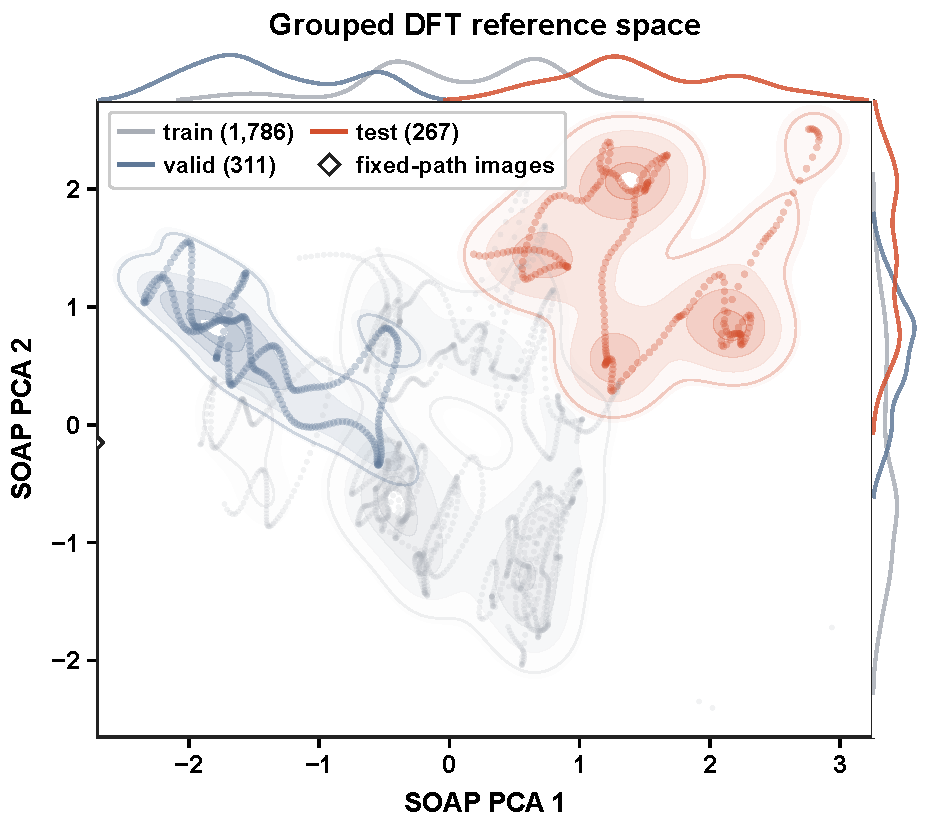
\includegraphics[width=0.82\textwidth]{analysis/task_conditioned_distribution_atlas_20261018/figures/fig_task_conditioned_panel_a.pdf}
\caption{\textbf{Grouped DFT reference space.} SOAP/PCA is fitted on the trajectory-grouped training partition only and applied without refitting to 1,786 training, 311 validation, 267 test, and five fixed-path images of the within-gap path G1. The training partition contains 1,783 periodic AIMD frames and three isolated-atom calibration frames; complete source AIMD trajectories are assigned to one partition. Soft two-dimensional density surfaces and calibrated marginal supports show the grouped split, while diamonds identify the fixed-path images. The latter are kept as a separate geometry class because the audited G1 images contain 61 atoms, whereas the grouped AIMD cells contain 81--86 atoms.}
\label{fig:task_conditioned_panel_a}

\end{figure*}

\begin{figure*}[t]
\centering
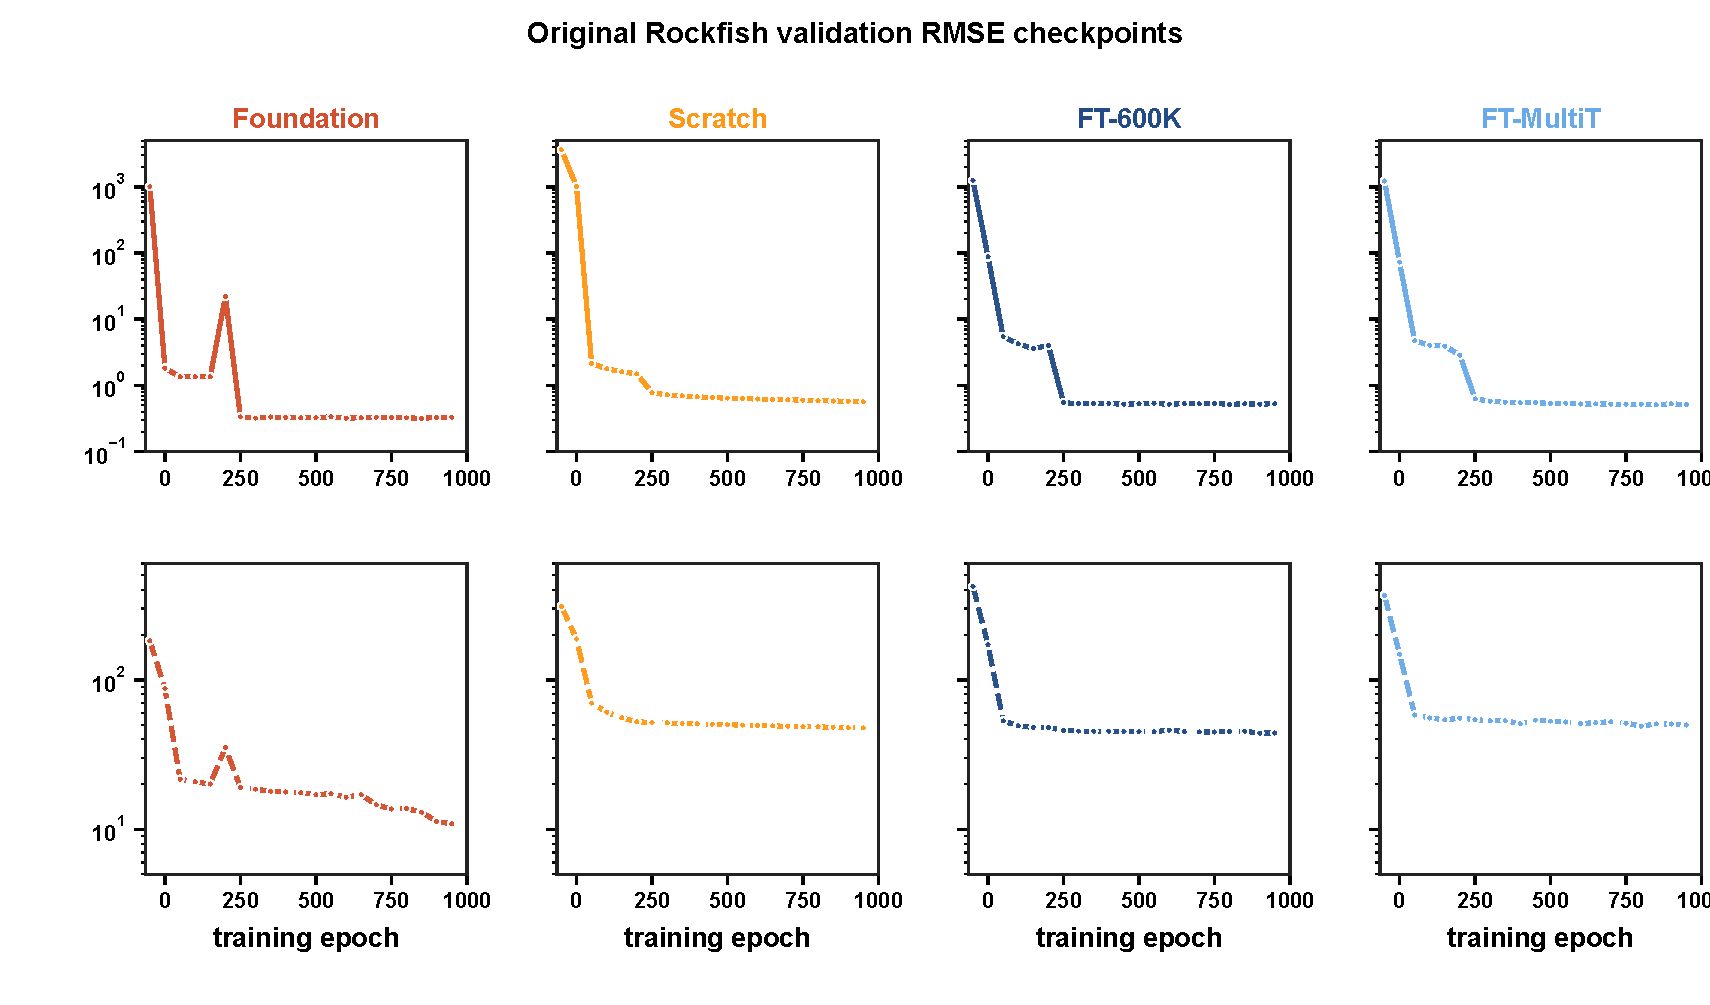
\includegraphics[width=0.98\textwidth]{analysis/task_conditioned_distribution_atlas_20261018/figures/fig_original_training_rmse_four_model.pdf}
\caption{\textbf{Validation RMSE during training.} The four columns follow the order Foundation, Scratch, FT-600K, and FT-MultiT. The upper row reports energy RMSE per atom and the lower row reports force RMSE, both converted from the original JSONL training logs to meV-based units. Each curve contains the unique default-head \texttt{mode=eval} checkpoints from the corresponding run~123 log; duplicate log checkpoints are retained in the raw table but omitted from the plotted trace. The curves are single-run validation histories from the original training campaigns. Source paths and SHA256 values are recorded in the accompanying RMSE manifest.}
\label{fig:original_training_rmse_four_model}

\end{figure*}

\begin{figure*}[t]
\centering
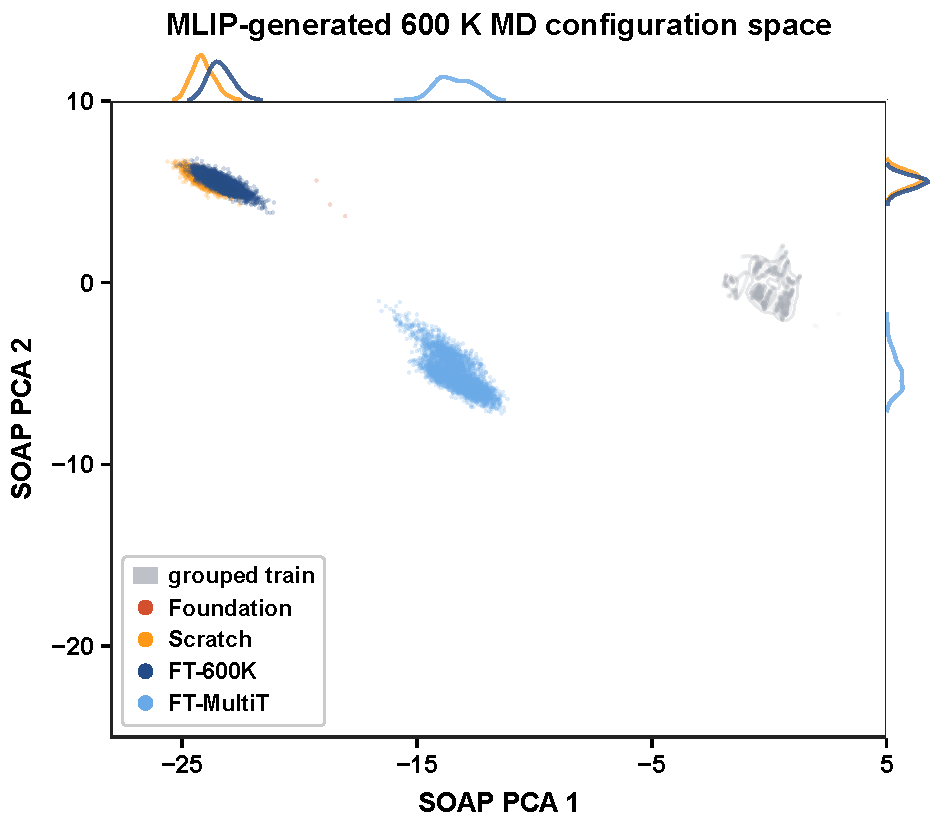
\includegraphics[width=0.82\textwidth]{analysis/task_conditioned_distribution_atlas_20261018/figures/fig_task_conditioned_panel_c.pdf}
\caption{\textbf{MLIP-generated 600~K MD configuration space.} SOAP/PCA distributions from the stored MLIP-generated continuation segments are overlaid on the grouped-training density using the same PCA transform as panel~(a). The stored rows are Foundation 4,961 (3 SOAP-valid and 4,958 short-contact skips), Scratch 4,001 (1,310 valid and 2,691 short-contact skips), FT-600K 4,601 valid, and FT-MultiT 4,001 valid. Short-contact rows (minimum interatomic distance below 1.2~\AA) are excluded from SOAP. The MD branches share a common velocity seed.}
\label{fig:task_conditioned_panel_c}

\end{figure*}
